% Made up for the tikra benchmark.
% The seven bridges of Konigsberg, and Euler's graph of them: four land masses, seven edges,
% every vertex of odd degree, so no walk crosses each bridge exactly once.
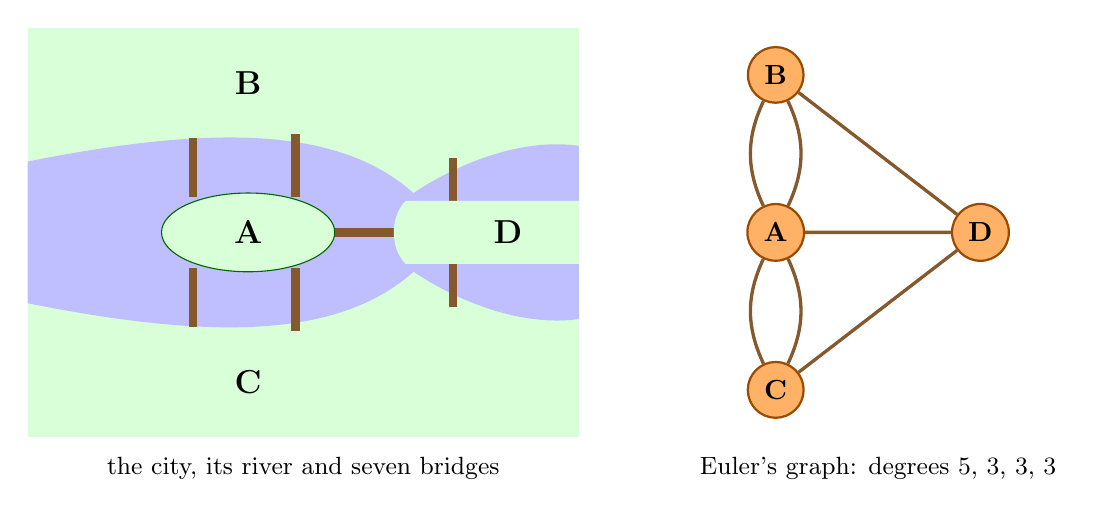
\begin{tikzpicture}[land/.style={circle, fill=orange!60, draw=orange!60!black, thick, minimum size=7mm, font=\bfseries}]
  % the map
  \begin{scope}
    \fill[green!15] (-0.5,-2.6) rectangle (6.5,2.6);
    \fill[blue!25] (-0.5,0.9) .. controls (2,1.4) and (3.5,1.3) .. (4.4,0.5) .. controls (5,0.9) and (5.8,1.2) .. (6.5,1.1)
      -- (6.5,-1.1) .. controls (5.8,-1.2) and (5,-0.9) .. (4.4,-0.5) .. controls (3.5,-1.3) and (2,-1.4) .. (-0.5,-0.9) -- cycle;
    \fill[green!15, draw=green!40!black] (2.3,0) ellipse (1.1 and 0.5);
    \foreach \x/\y/\a in {1.7/0.45/90, 2.9/0.45/90, 1.7/-0.45/90, 2.9/-0.45/90, 2.3/0/0, 4.4/0.75/90, 4.4/-0.75/90} {}
    \foreach \p/\q in {{(1.6,0.45)}/{(1.6,1.2)}, {(2.9,0.45)}/{(2.9,1.25)}, {(1.6,-0.45)}/{(1.6,-1.2)}, {(2.9,-0.45)}/{(2.9,-1.25)},
        {(3.4,0)}/{(4.3,0)}, {(4.9,0.25)}/{(4.9,0.95)}, {(4.9,-0.25)}/{(4.9,-0.95)}}
      \draw[brown!70!black, line width=3pt] \p -- \q;
    \fill[green!15] (4.3,-0.4) -- (6.5,-0.4) -- (6.5,0.4) -- (4.3,0.4) .. controls (4.1,0.2) and (4.1,-0.2) .. (4.3,-0.4);
    \node[font=\large\bfseries] at (2.3,0) {A}; \node[font=\large\bfseries] at (2.3,1.9) {B};
    \node[font=\large\bfseries] at (2.3,-1.9) {C}; \node[font=\large\bfseries] at (5.6,0) {D};
    \node[font=\small] at (3,-3) {the city, its river and seven bridges};
  \end{scope}
  % Euler's graph
  \begin{scope}[xshift=9cm]
    \node[land] (A) at (0,0) {A}; \node[land] (B) at (0,2) {B};
    \node[land] (C) at (0,-2) {C}; \node[land] (D) at (2.6,0) {D};
    \draw[very thick, brown!70!black] (A) to[bend left=25] (B) (A) to[bend right=25] (B)
      (A) to[bend left=25] (C) (A) to[bend right=25] (C) (A) -- (D) (B) -- (D) (C) -- (D);
    \node[font=\small, align=center] at (1.3,-3) {Euler's graph: degrees 5, 3, 3, 3};
  \end{scope}
\end{tikzpicture}
